\documentclass[9pt,twocolumn,twoside,lineno]{pnas-new}
% Use the lineno option to display guide line numbers if required.

\usepackage{siunitx}

\templatetype{pnasresearcharticle} % Choose template 
% {pnasresearcharticle} = Template for a two-column research article
% {pnasmathematics} %= Template for a one-column mathematics article
% {pnasinvited} %= Template for a PNAS invited submission

\title{A multi-control climate policy process for a designated decision maker}

% Use letters for affiliations, numbers to show equal authorship (if applicable) and to indicate the corresponding author
\author[a,b,1]{Henri F. Drake}
\author[a]{Ronald L. Rivest} 
\author[a]{Alan Edelman}
\author[a]{John Deutch}

\affil[a]{Massachusetts Institute of Technology, 77 Massachusetts Ave, Cambridge, MA 02139, USA}
\affil[b]{MIT-WHOI Joint Program in Oceanography/Applied Ocean Science \&
Engineering, Cambridge and Woods Hole, MA, 02139, USA}

% Please give the surname of the lead author for the running footer
\leadauthor{Drake} 

% Please add a significance statement to explain the relevance of your work
\significancestatement{Authors must submit a 120-word maximum statement about the significance of their research paper written at a level understandable to an undergraduate educated scientist outside their field of speciality. The primary goal of the significance statement is to explain the relevance of the work in broad context to a broad readership. The significance statement appears in the paper itself and is required for all research papers.}

% Please include corresponding author, author contribution and author declaration information
\authorcontributions{All authors contributing to the conception of the project, interpretation of the results, and writing of the paper. HFD ran the simulations and created the figures.}
\authordeclaration{Please declare any competing interests here.}
\correspondingauthor{\textsuperscript{1}To whom correspondence should be addressed. E-mail: henrifdrake@gmail.com}

% At least three keywords are required at submission. Please provide three to five keywords, separated by the pipe symbol.
\keywords{Climate policy $|$ Integrated Assessment Model $|$ Mitigation $|$ Adaptation $|$ Geoengineering}

\begin{abstract}
Please provide an abstract of no more than 250 words in a single paragraph. Abstracts should explain to the general reader the major contributions of the article. References in the abstract must be cited in full within the abstract itself and cited in the text.
\end{abstract}

\dates{This manuscript was compiled on \today}
\doi{\url{www.pnas.org/cgi/doi/10.1073/pnas.XXXXXXXXXX}}

\begin{document}

\maketitle
\thispagestyle{firststyle}
\ifthenelse{\boolean{shortarticle}}{\ifthenelse{\boolean{singlecolumn}}{\abscontentformatted}{\abscontent}}{}

% If your first paragraph (i.e. with the \dropcap) contains a list environment (quote, quotation, theorem, definition, enumerate, itemize...), the line after the list may have some extra indentation. If this is the case, add \parshape=0 to the end of the list environment.
\dropcap{T}his PNAS journal template is provided to help you write your work in the correct journal format. Instructions for use are provided below. 

Note: please start your introduction without including the word ``Introduction'' as a section heading (except for math articles in the Physical Sciences section); this heading is implied in the first paragraphs. 

\section*{MARGO: An idealized model of optimally-controlled climate change}

The \textbf{MARGO} model consists of a physical energy balance model of Earth's climate coupled to an idealized socio-economic model of climate damages and controls:
\begin{center}
\begin{tabular}{l}
\textbf{M}itigation of greenhouse gas emissions, \\
\textbf{A}daptation to climate impacts, \\
\textbf{R}emoval of carbon dioxide, \\
\textbf{G}eoengineering by solar radiation management, and\\
\textbf{O}ptimal deployment of available controls.
\end{tabular}
\end{center}
The model is modular, fast, and customizable and can be run with several options of objective functions and constraints.

Each of the climate controls acts, in its own distinct way, to reduce the damages caused by a changing climate but also carry their own deployment costs (including direct costs, research and development costs, infrastructure costs, regulatory costs). The model is designed to include key features of climate physics, economics, and policy as concisely as possible and in ways consistent with both theory and more comprehensive General Circulation and Integrated Assessment Models. The shortcoming of the model's simplicity is that while its results provide qualitative insights, the quantitative results are unreliable predictions.

The model is developed in open source using the Julia programming language \cite{bezanson_julia:_2017} at \url{github.com/hdrake/OptimizeClimate} (Drake et al., 2020). The parameter values used throughout the paper are set to the defaults reported in Section 1 of the Supplemental Information, except where explicitly stated otherwise. In Section 2 of the Supplementary Information, we show that by tweaking just a few of these default parameter values, the model replicates the qualitative results of studies ranging from analytical control theory analysis of solar-geoengineering deployments \cite{soldatenko_optimal_2018} to numerical optimizations of mitigation, carbon dioxide removal, and solar geo-engineering deployments in DICE, a commonly used Integrated Assessment Model \cite{belaia_optimal_2019}.

\subsection*{No-policy baseline scenario}
Climate-controlled scenarios are considered relative to an exogenous no-policy baseline where carbon-dioxide equivalent (CO$_{2e}$) emissions $q(t)$ increase four-fold by 2100 and decrease to zero by 2150, resulting in $\SI{7.3}{W/m^{2}}$ of radiative forcing by 2100 and $\SI{8.5}{W/m^{2}}$, which we interpret as an idealized extension of the SSP3 baseline scenario characterized by nationalistic fossil-fueled growth \cite[][and Section A of Supplemental Information]{riahi_shared_2017}.

There are five steps in the causal chain between CO$_{2e}$ emissions and climate damages.
\begin{enumerate}
    \item CO$_{2e}$ is emitted at a rate $q(t)$, with only $r = 50\%$ remaining in the atmosphere net of uptake by the ocean and terrestrial biosphere (Figure \ref{fig:carbon_and_temperature}a).
    \item CO$_{2e}$ concentrations increase as long as the emissions $q(t)$ are non-zero and are given by $c(t) = c(t_{0}) + \int_{t_{0}}^{t} rq(t)\text{ d}t$ (Figure \ref{fig:carbon_and_temperature}b).
    \item Increasing CO$_{2e}$ concentrations strengthen the greenhouse effect, reducing outgoing longwave radiation and causing an increased radiative forcing of $F(t) = a \ln(c(t)/c_{t_{0}})$. 
    \item Near-surface air temperatures increase by $T(t) = F(t)/B$ to balance the reduced cooling to space, where a fraction $B/(\kappa + B)$ of the warming occurs within a few years and the remaining fraction $\kappa/(B + \kappa)$ occurs over the course of several centuries due to ocean heat uptake. The feedback parameter $B$ includes the effects of all climate feedbacks, except those involving the carbon cycle and the long-term ice sheet response (Figure \ref{fig:carbon_and_temperature}c), and the ocean heat uptake rate $\kappa$ parameterizes the combined effects of advection and diffusion of heat into the deep ocean.
    \item Anthropogenic warming causes a myriad of climate impacts, which result in damages that increase non-linearly with temperature, $D = \beta T^{2}$.
\end{enumerate} 

\subsection*{Effects of climate controls}

The four available climate controls enter as fractional controls at each link of the climate change causal chain \cite[similar to][]{moreno-cruz_economic_2018}:
\begin{equation}
    \text{Emission}
    \xrightarrow{\text{\textbf{M}}}
    \text{CO$_{2e}$}
    \xrightarrow{\text{\textbf{R}}}
    \text{Forcing}
    \xrightarrow{\text{\textbf{G}}}
    \text{Warming}
    \xrightarrow{\text{\textbf{A}}}
    \text{Damage}
\end{equation}

\begin{figure*}%[tbhp]
\centering
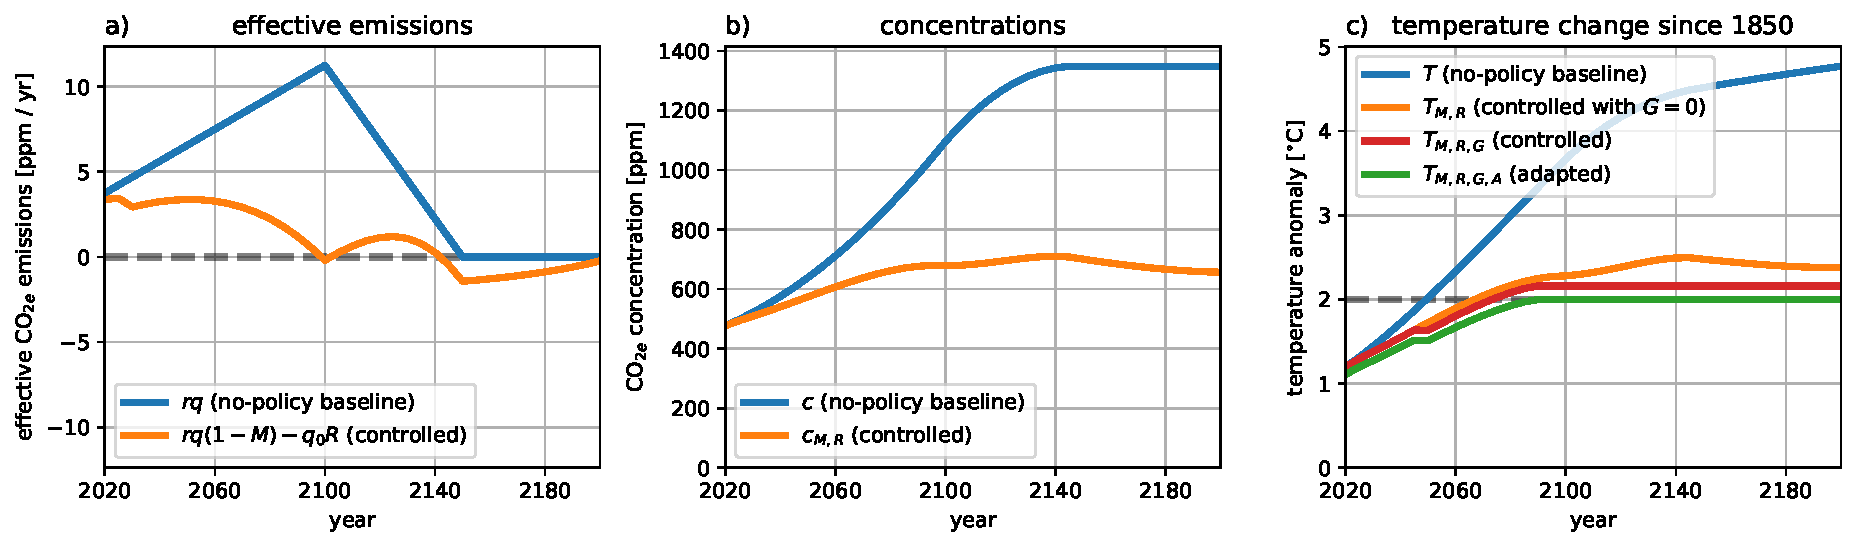
\includegraphics[width=17.8cm]{figures/default-temp_carbon_and_temperatures.pdf}
\caption{Baseline (blue) and optimally-controlled (orange) a) effective CO$_{2e}$ emissions, b) CO$_{2e}$ concentrations, and c) temperature anomaly relative to preindustrial from cost-effectiveness analysis (see Section \ref{sec:cost-effectivness}). Panel c) shows the optimal temperature change that would occur: in a baseline scenario (blue); with just emissions \textbf{M}itigation and carbon dioxide \textbf{R}emoval (orange); with \textbf{M}itigation, \textbf{R}emoval, and solar-\textbf{G}eoengineering (red); and as an ``adapted temperature" (eq. \ref{eq.adapted_temperature}) with \textbf{A}daptation measures also taken into account. The dashed grey line marks the threshold adapted temperature of $T^{\star} = \SI{2}{\celsius}$ to be avoided.}
\label{fig:carbon_and_temperature}
\end{figure*}

\textbf{M}itigation reduces emissions by a factor $M(t) \in [0,1]$ such that the controlled emissions that remain in the atmosphere are $rq(t)\,(1-M(t))$, where $M = 1$ corresponds to complete decarbonization of the economy.

\textbf{R}emoval of CO$_{2e}$, $R(t) \in [0,1]$, in contrast to mitigation, is de-coupled from instantaneous emissions and is expressed as the fraction of 2020 baseline emissions that are removed from the atmosphere in a given year, $q_{0}R(t)$. A maximal value of $R=1$ corresponds to removing $\SI{59}{GtCO_{2e} / year}$, which is more than twice a median estimate of the global potential for negative emission technologies \cite{fuss_negative_2018}.

A useful diagnostic quantity is the effective emissions
\begin{equation}
    rq(t)(1-M(t)) - q_{0}R,
    \label{eq:effective-emissions}
\end{equation} which is the annual rate of $CO_{2e}$ accumulation in the atmosphere (Figure \ref{fig:carbon_and_temperature}a) and is controlled by both mitigation and carbon dioxide removal.
The CO$_{2e}$ concentration is simply the integral of the effective emissions over time (Figure \ref{fig:carbon_and_temperature}b),
\begin{equation}
    c_{M,R}(t) = c_{0} + \int_{t_{0}}^{t} rq(t')(1-M(t')) \text{ d}t' - q_{0} \int_{t_{0}}^{t} R(t')\text{ d}t'.
\end{equation}

\textbf{G}eoengineering by solar radiation management, $G(t) \in [0,1]$, acts to offset a fraction of the CO$_{2e}$ forcing, 
\begin{equation}
    F_{M,R,G}(t) = F_{M,R}(t) - G(t) F(t \rightarrow \infty),
\end{equation}
where $F_{M,R} = a \ln(c_{M,R}(t) / c_{0})$ is the controlled CO$_{2e}$ forcing and $F(t \rightarrow \infty) = \SI{8.5}{W/m^{2}}$ is the maximum baseline CO$_{2e}$ forcing, which is attained starting in 2150. A value of $G = 1$ thus corresponds to a complete cancellation between the baseline equilibrium warming by CO$_{2e}$ and cooling by reflecting incoming solar radiation.

The controlled near-surface air temperature (Figure \ref{fig:carbon_and_temperature}c) evolves according to the total controlled forcing,
\begin{equation}
    T_{M,R,G}(t) - T_{0} = \frac{F_{M,R,G}(t)}{B + \kappa} + \frac{\kappa}{B} \int_{t_{0}}^{t} \frac{e^{\frac{t'-t}{\tau_{D}}}}{\tau_{D}} \frac{F_{M,R,G}(t')}{B+\kappa} \, \text{d}t',
    \label{eq:temperature}
\end{equation}
where $T_{0} = \SI{1.1}{\celsius}$ is the present warming relative to preindustrial and $\tau_{D} = \SI{240}{years}$ is the slow timescale of ocean heat uptake. The first term on the right-hand side of [\ref{eq:temperature}] represents a fast transient response while the second term represents a slow recalcitrant response due to the thermal inertia of the deep ocean. Climate inertia decouples the temperature response from instantaneous forcing and implies that a certain amount of warming is locked in for the future, even if radiative forcing is stabilized (as in the case of bring emissions to zero in our model\footnote{In earth system models with a dynamic carbon cycle, the slow recalcitrant warming due to a reduction in ocean heat uptake happens to be roughly offset by the ocean carbon sink \cite{solomon_irreversible_2009,lickley_time_2019}, such that bringing emissions to zero roughly stabilizes temperatures.}).

\textbf{A}daptation to climate impacts acts to reduce damages by a fraction $A(t) \in [0, 1/3]$. Since some climate impacts are likely impossible to adapt to \cite[][]{sherwood_adaptability_2010}, we assume that adaptation can at most reduce climate damages by one-third. The controlled damages are thus given by
\begin{equation}
    D_{M,R,G,A} = \beta (T_{M,R,G})^{2} (1-A(t)),
    \label{eq:damages}
\end{equation}
where the damage parameter $\beta$ is tuned such that a warming of $\SI{3}{\celsius}$ results in damages of the $2\%$ of Global World Product (GWP). Although adaptation does not affect the planetary temperature directly, it is useful to consider an "adapted temperature" $T_{M,R,G,A}$ which yields controlled damages equivalent to the fully-controlled damages $\beta (T_{M,R,G,A})^{2} = \beta (T_{M,R,G})^{2} (1-A)$ and is defined
\begin{equation}
    T_{M,R,G,A} \equiv T_{M,R,G} \sqrt{(1-A)}.\label{eq:adapted-temperature}
\end{equation}

\subsection*{Costs and benefits of controlling the climate}

The costs of deploying climate controls are non-negligible and must in some way be balanced with the benefits of controlling to climate to avoid damages. The costs of climate controls are parameterized as:
\begin{equation}
    \mathcal{C} = \mathcal{C}_{M} M^{2} + \mathcal{C}_{R} R^{2} + \mathcal{C}_{G} G^{2} + \mathcal{C}_{A} A^{2},
\end{equation}
where the $C_{*}$ are the hypothetical annual costs of fully deploying that control, the values of which are justified in the Methods.

The benefits of deploying climate controls are the avoided climate damages relative to the no-policy baseline scenario,
\begin{equation}
    \mathcal{B} = D - D_{M,R,G,A} = \beta (T^{2} - (T_{M,R,G,A})^{2}).
\end{equation}

\subsection*{Exogenous economic growth}
In contrast to conventional Integrated Assessment Models, which follow classic economic theories of optimal economic growth and solve for the maximal welfare based on the discounted utility of consumption, we here treat economic growth as exogenous. The economy $E(t) = E_{0}(1 + \gamma)^{(t-t_{0})}$ grows from its present value of $E_{0} = \SI{100}{\,trillion\, USD}$ with a fixed growth rate $\gamma = 2\%$, which approximates the economic growth in various simulations of DICE2013r \cite{nordhaus2013dice}. We ignore feedbacks of climate abatement costs and climate damages on economic growth, since they are small variations relative to the exponential rate of economic growth in conventional Integrated Assessment Models \cite{nordhaus2013dice}.

\section*{Optimal deployments of climate controls}

If a trusted climate policy decision-maker specifies an objective function to maximize and, optionally, additional policy constraints, the MARGO model is readily optimized in terms of the time-dependent climate control variables $M(t), R(t), G(t), A(t)$. The numerical implementation of the optimization, as well as additional constraints on the permitted rates of deployments, are described in the Methods. Here, we describe the optimally-controlled results of two policy approaches, cost-benefit analysis and cost-effectiveness analysis, and explore their sensitivity to the discount rate $\rho$ and possible limits to the fractional penetration of mitigation $\mu$, respectively.

\subsection*{Cost-benefit analysis}\label{sec:cost-benefit}

A natural and widely-used objective function is the cost-benefit framework, in which the cost $\mathcal{C}_{M, R, G, A}$ of deploying climate controls is balanced against the benefits $\mathcal{B}_{M, R, G, A}$ of the avoided climate damages. Formally, we aim to maximize the net present benefits:
\begin{gather}
    \max \left\{ \int_{t_{0}}^{t_{f}} 
    \left(\mathcal{B}_{M, R, G, A} - \mathcal{C}_{M, R, G, A} \right) (1 + \rho)^{-(t-t_{0})} \, \text{d}t \right\},
    \label{eq.net_present_benefits}
\end{gather}
where $\rho$ is a discount rate that determines the annual depreciation of future costs and benefits. There are different views about the appropriate non-zero discount rate to apply to multi-generational social utility \cite{ramsey_mathematical_1928, solow_economics_1974, stern_economics_2007}. Here, we choose a discount rate of $\rho = 1\%$, on the low end of values used in the literature, motivated by our preference towards inter-generational equity\footnote{Follow \cite{stern_economics_2007}'s discussion of the discount rate...}.

The results of maximizing net benefits are shown in Figure \ref{fig:cost-benefit}. Early and aggressive emissions mitigation– and to a lesser extent carbon dioxide removal (Fig \ref{fig:cost-benefit}a)– carry net costs of up to 1 trillion USD/year before 2050 relative to the no-policy baseline but deliver orders of magnitude more in benefits from 2050 to 2200 (Fig \ref{fig:cost-benefit}b). Deployments of adaptation and solar-geoengineering are relatively modest, reflecting their relative high costs and the fact that they are further down the causal chain of climate damages and do not directly affect the root cause of the damage: increasing CO$_{2e}$ concentrations due to positive effective emissions.

The preference for controls earlier in the causal chain, notably mitigation, is largely a result of our subjective choice $\rho = 1\%$ for the discount rate. In particular, as the discount rate increases above the economic growth rate, $\rho > \gamma = 2\%$, the decay of the discount factor out-competes economic growth and leads to a different regime of control preferences: the short-term fix offered by solar geo-engineering becomes the dominant control since the high future costs of its unintended damages are effectively annulled by the aggressive discounting.

\begin{figure*}%[tbhp]
\centering
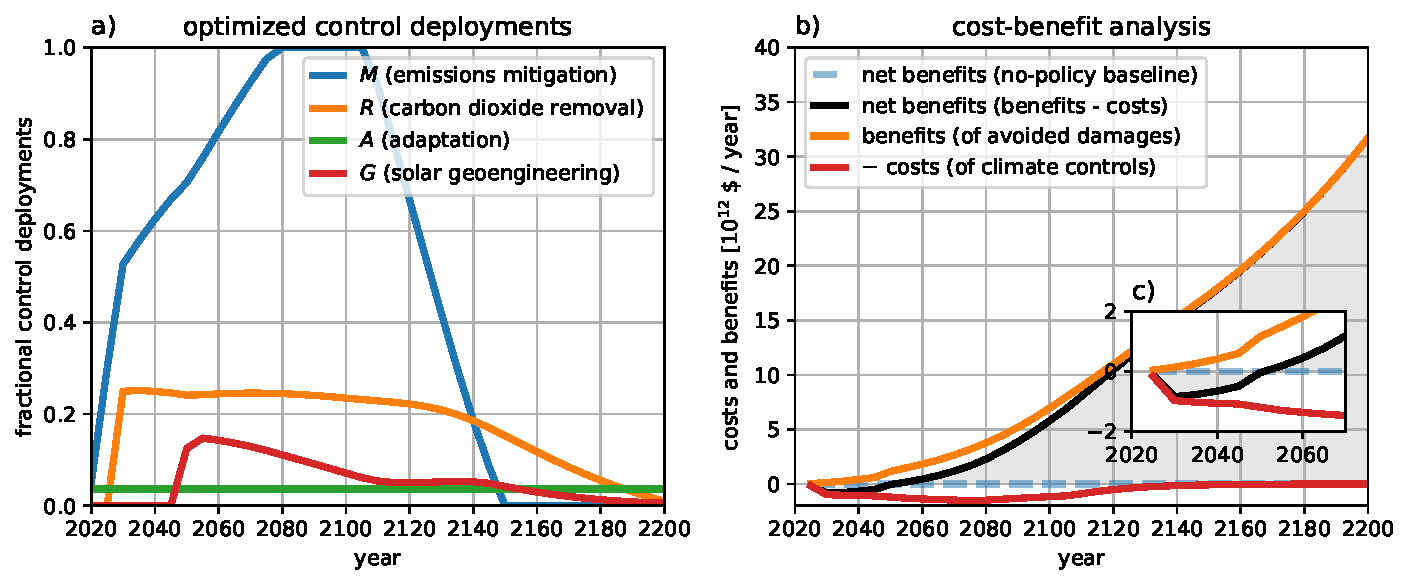
\includegraphics[width=17.8cm]{figures/default-benefits_controls_and_benefits.pdf}
\caption{Results of cost-benefit analysis and sensitivity to the discount rate $\rho$. (a) Optimal control deployments and (b) corresponding discounted costs and benefits relative to the no climate-policy baseline scenario. The total positive area shaded in grey in (b) is the maximal net present benefits (eq. \ref{eq:net-present-benefits}). An inset zooms in on the 2020 to 2050 period of modest net costs. (c) Time-mean control deployments as a function of the discount rate.}
\label{fig:cost-benefit}
\end{figure*}

\subsection*{Cost-effectiveness of avoiding damage thresholds}\label{sec:cost-effectivness}

The conventional cost-benefit approach to understanding climate change is limited by the poorly constrained damage function, which has historically been under-estimated \cite{} and must be continually revised as we understand more about climate surprises lurking at high levels of forcing \citep{alley_abrupt_2003, sherwood_adaptability_2010, scher_carbonocean_2017}. An alternative approach, which presently guides global climate policy negotiations, is to prescribe a threshold of climate damages– or temperatures, as in the Paris Climate Agreement \cite{ParisAgreement2015} - which is not to be surpassed.

In our implementation of the cost-effectiveness approach, we aim to find the lowest net present costs of control deployments
\begin{equation}
    \min\left\{\int_{t_{0}}^{t_{f}} \mathcal{C}_{M,R,G,A} (1 + \rho)^{-(t-t_{0})} \text{ d}t\right\}
\end{equation}
which keep controlled damages below the level corresponding to a chosen temperature threshold,
$\beta (T_{M,R,G})^{2} (1 - A(t)) < \beta (T^{\star})^{2}$, which we rewrite
\begin{equation}
    T_{M,R,G,A} < T^{\star},
\end{equation}
where $T_{M,R,G,A}$ is the "adapted temperature" (eq. \ref{eq:adapted-temperature}) and the threshold $T^{\star} = \SI{2}{\celsius}$ is inspired by the Paris Climate Agreement.

The results of optimizing the cost-effectiveness of controls that keep adapted temperatures below $T^{\star} = \SI{2}{\celsius}$ are shown in Figures \ref{fig:carbon_and_temperature} and \ref{fig:cost-effectiveness}. Fractional emissions mitigation increases proportional to the increase in baseline emissions, reaching $M=\SI{90}{\%}$ decarbonization by 2100, while carbon dioxide is removed at a roughly constant rate of $R q_{0} \approx 20\%\, q_{0} = \SI{1.5}{ppm/year}$ starting in 2030. Since the optimally-controlled temperatures that result from the above cost-benefit analysis are already lower than $T^{\star}$, the optimal controls from cost-effectiveness are less ambitious than for the cost-benefit analysis (Figures \ref{fig:cost-benefit}a, \ref{fig:cost-effectiveness}a). As a consequence of relatively relaxed mitigation and carbon dioxide removal early on, small but non-negligible deployment of solar-geoengineering is used to shave off a few tenths of a degree of warming during its peak in the mid-22nd Century in order to meet the temperature goal (Figure \ref{fig:cost-effectiveness}a and Figure \ref{fig:carbon_and_temperature}c). Adaptation offsets $A = \SI{15}{\%}$ of damages and plays a moderate role in reducing damages below the threshold. Even after discounting, annual costs of control deployments peak in 2100, driven by a peak in mitigation, which is most cost-efficient in 2100 where the baseline emissions are the highest (Figure \ref{fig:cost-effectiveness}b).

To explore the sensitivity of these results to our assumed mitigation costs $\mathcal{C}_{M} M^{2}$, which allow for up to $90\%$ mitigation in 2100 at the relatively low cost of $\SI{1.6}{trillion\; USD/year}$ ($\SI{7}{USD/tCO_{2e}}$), we add the multiplicative factor for penetration $P(\mu) = \left(1 - e^{20(M-\mu)}\right)^{-1}$ to the mitigation cost function. The penetration factor $P(\mu)$ is equal to $1$ except in the vicinity of $M = \mu$, where it rapidly asymptotes to infinity (Figure \ref{fig:cost-effectiveness}d). The original cost function is recovered in the limit $\mu \gg 1$. As we lower the penetration limit $\mu$ of mitigation, the . Maximum solar geo-engineering is relatively constant for high $\mu$ but begins to increase as $\mu < 25\%$. FINISH THIS SECTION!!!


\begin{SCfigure*}%[tbhp]
\centering
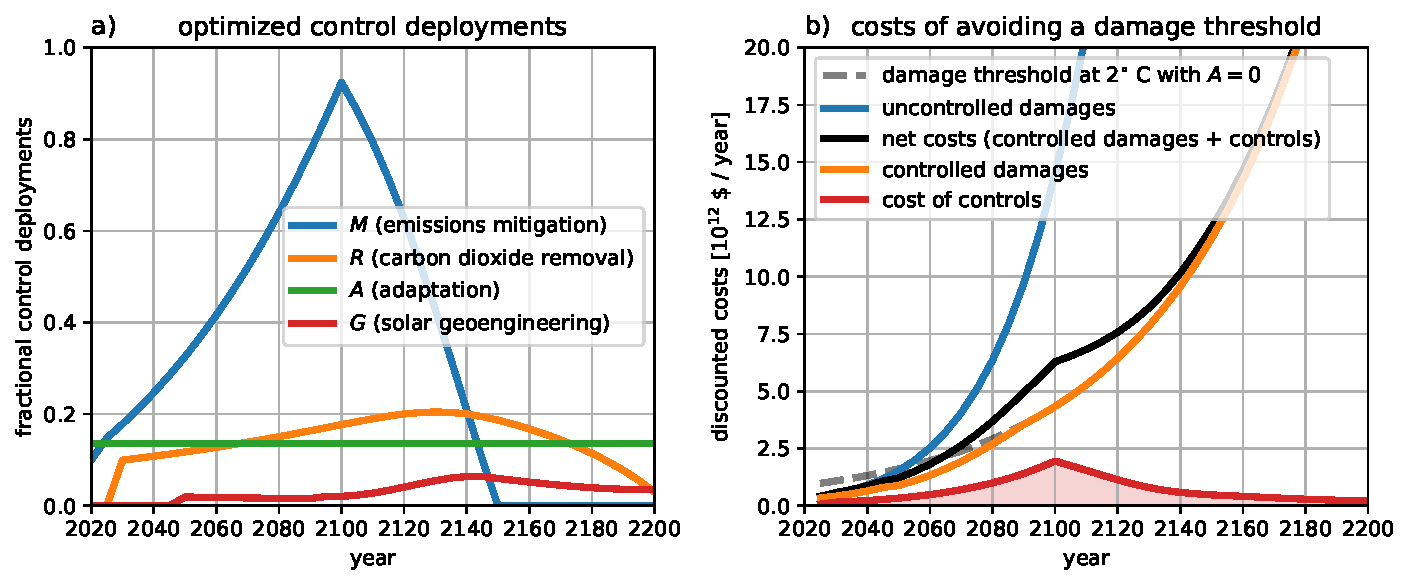
\includegraphics[width=11.4cm]{figures/default-temp_controls_and_damages.pdf}
\caption{Results of cost-benefit analysis and sensitivity to potential limits $\mu$ to mitigation. (a) Optimal control deployments and (b) corresponding costs and damages. In panel (b), the blue line shows the discounted baseline uncontrolled damages; the dashed grey line shows the discounted damages associated with $2^{\circ}$ of warming, which are to be avoided at all costs; the orange line shows the discounted damages in the optimally-controlled solution; and the red line shows the optimal discounted costs of controls such that the shaded area below is the minimal net present costs of controls (eq. \ref{eq:cost-effectiveness}). (c) The maximum deployment of each control as a function of $\mu$, the mitigation level at which costs asymptote to infinity, where the mitigation cost function has been modified to the asymptotic function $\mathcal{C}_{M} M^{2} \left( 1 - e^{20 (M - \mu)} \right)^{-1}$ shown in (d) for three values of $\mu$.}
\label{fig:cost-effectiveness}
\end{SCfigure*}

\section*{A policy process for responding to uncertain future outcomes}


\begin{SCfigure*}%[tbhp]
\centering
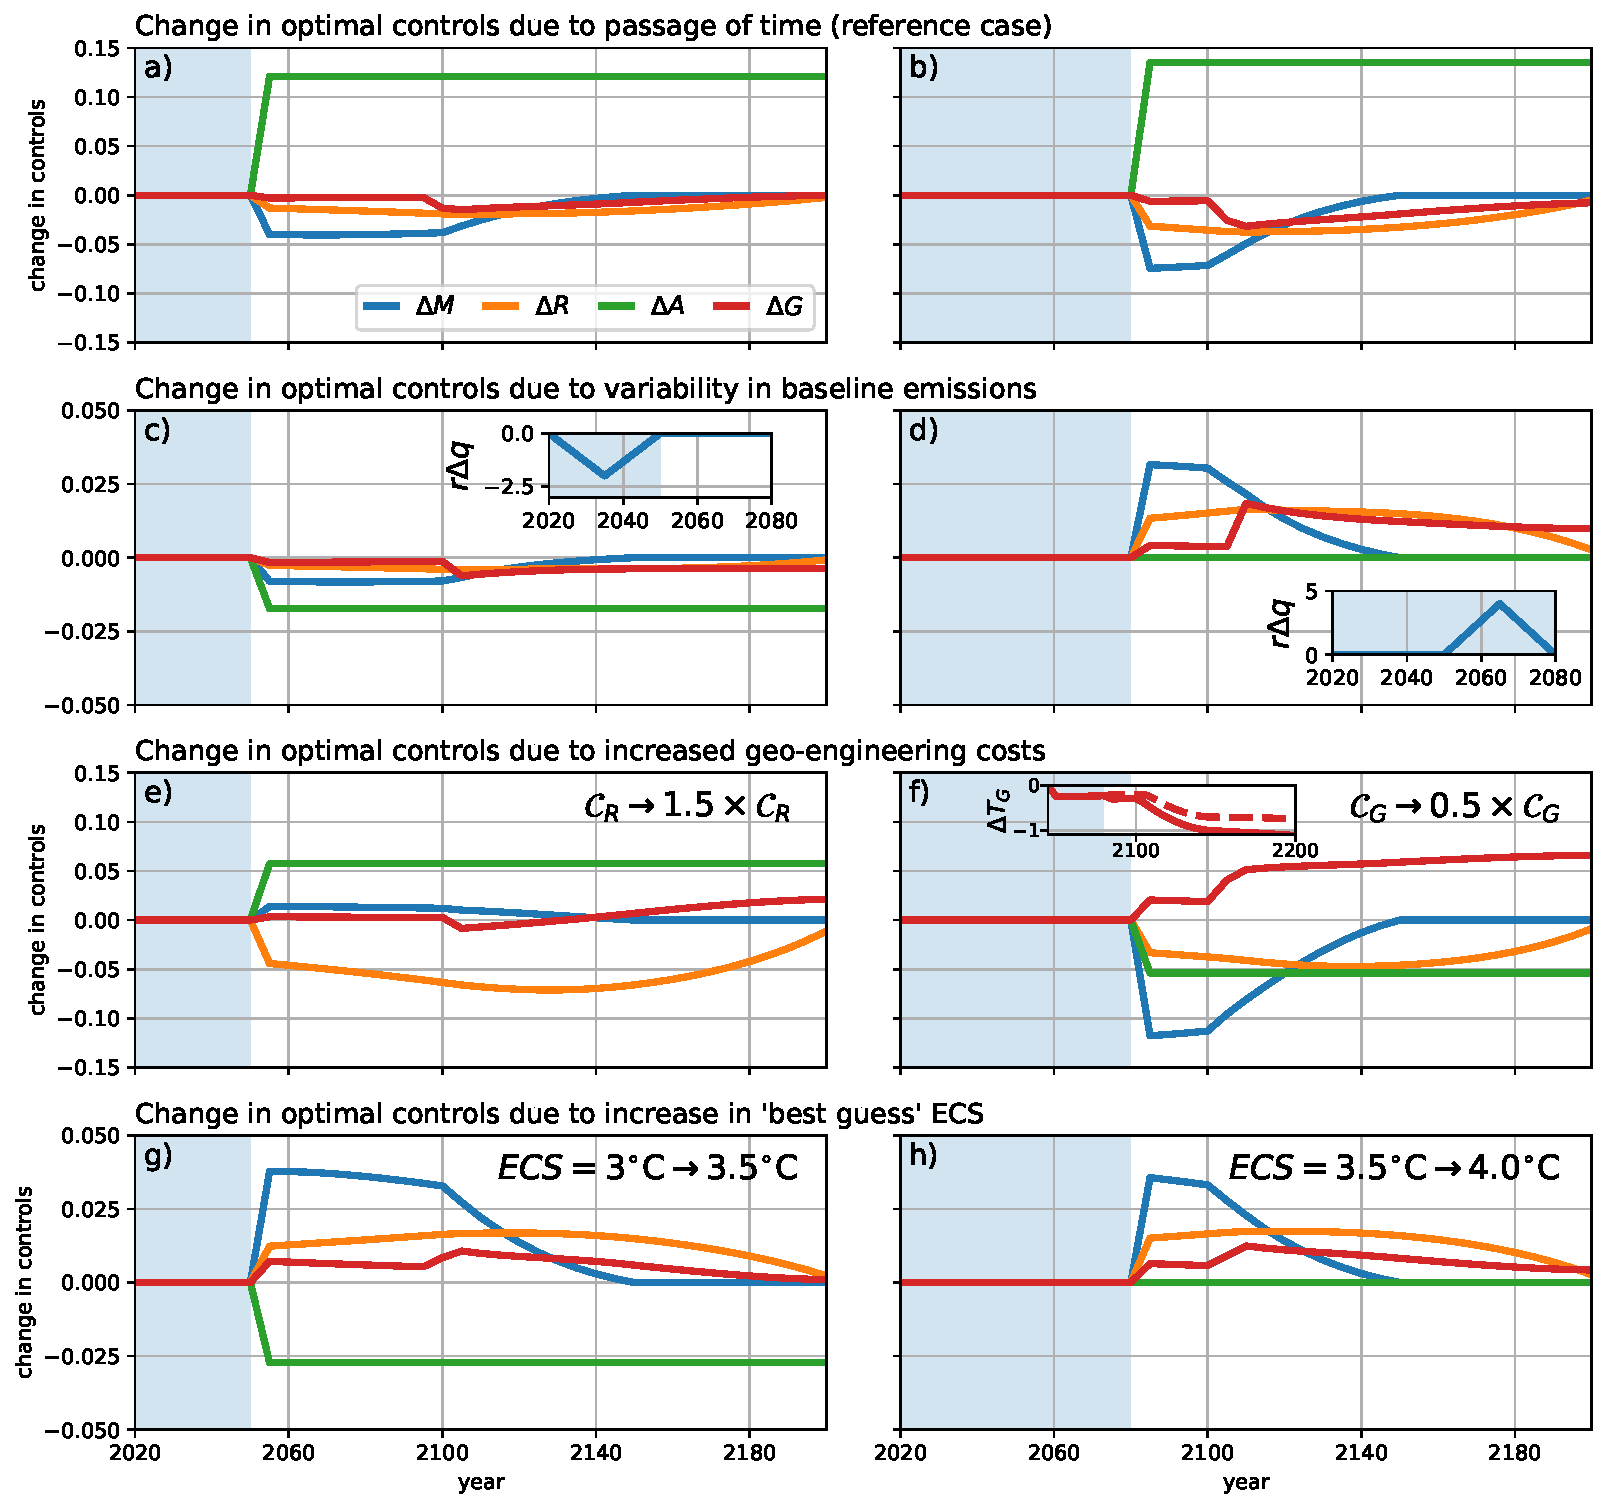
\includegraphics[width=11.4cm]{figures/policy_updates.pdf}
\caption{Illustration of a proposed responsive policy progress. (a) Optimal climate control trajectories for avoiding $T^{\star} = \SI{2}{\celsius}$ of warming, as in Figure \ref{fig:cost-effectiveness}a. (b) Baseline and optimally-controlled effective emissions, as well as the hypothetical variability in baseline emissions considered in panels (c) and (d). (c-h) Difference in optimal control trajectories due to sequential re-optimization at 2050 and 2080 with revised model parameters: (c,d) where historical effective emissions $rq(t)$ are sequentially increased and then decreased (insets), (e,f) where the costs of carbon and solar geo-engineering are sequentially increased, and (g,h) where the best guess of the Equilibrium Climate Sensitivity (ECS) is revised upwards in 2050 and again in 2080.}
\label{fig:cost-effectiveness}
\end{SCfigure*}

\subsection*{Example: uncertainty in baseline emissions}

\subsection*{Example: uncertainty in geoengineering costs}

\subsection*{Example: uncertain in the climate sensitivity}

\section*{Discussion}

\subsection*{Author Affiliations}

Include department, institution, and complete address, with the ZIP/postal code, for each author. Use lower case letters to match authors with institutions, as shown in the example. Authors with an ORCID ID may supply this information at submission.

\subsection*{Submitting Manuscripts}

All authors must submit their articles at \href{http://www.pnascentral.org/cgi-bin/main.plex}{PNAScentral}. If you are using Overleaf to write your article, you can use the ``Submit to PNAS'' option in the top bar of the editor window. 

\subsection*{Format}

Many authors find it useful to organize their manuscripts with the following order of sections;  title, author line and affiliations, keywords, abstract, significance statement, introduction, results, discussion, materials and methods, acknowledgments, and references. Other orders and headings are permitted.

\subsection*{Manuscript Length}

A standard 6-page article is approximately 4,000 words, 50 references, and 4 medium-size graphical elements (i.e., figures and tables). The preferred length of articles remains at 6 pages, but PNAS will allow articles up to a maximum of 12 pages.

\subsection*{References}

References should be cited in numerical order as they appear in text; this will be done automatically via bibtex, e.g. \cite{belkin2002using} and \cite{berard1994embedding,coifman2005geometric}. All references cited in the main text should be included in the main manuscript file.

\subsection*{Data Archival}

PNAS must be able to archive the data essential to a published article. Where such archiving is not possible, deposition of data in public databases, such as GenBank, ArrayExpress, Protein Data Bank, Unidata, and others outlined in the \href{https://www.pnas.org/page/authors/journal-policies#xi}{Information for Authors}, is acceptable.

\subsection*{Language-Editing Services}
Prior to submission, authors who believe their manuscripts would benefit from professional editing are encouraged to use a language-editing service (see list at www.pnas.org/page/authors/language-editing). PNAS does not take responsibility for or endorse these services, and their use has no bearing on acceptance of a manuscript for publication. 

\subsection*{Digital Figures}

EPS, high-resolution PDF, and PowerPoint are preferred formats for figures that will be used in the main manuscript. Authors may submit PRC or U3D files for 3D images; these must be accompanied by 2D representations in TIFF, EPS, or high-resolution PDF format. Color images must be in RGB (red, green, blue) mode. Include the font files for any text.

Images must be provided at final size, preferably 1 column width (8.7cm). Figures wider than 1 column should be sized to 11.4cm or 17.8cm wide. Numbers, letters, and symbols should be no smaller than 6 points (2mm) and no larger than 12 points (6mm) after reduction and must be consistent. 

Figures and tables should be labelled and referenced in the standard way using the \verb|\label{}| and \verb|\ref{}| commands.

Figure \ref{fig:frog} shows an example of how to insert a column-wide figure. To insert a figure wider than one column, please use the \verb|\begin{figure*}...\end{figure*}| environment. Figures wider than one column should be sized to 11.4 cm or 17.8 cm wide. Use \verb|\begin{SCfigure*}...\end{SCfigure*}| for a wide figure with side legends.

\subsection*{Tables}
Tables should be included in the main manuscript file and should not be uploaded separately.

\subsection*{Single column equations}

Authors may use 1- or 2-column equations in their article, according to their preference.

To allow an equation to span both columns, use the \verb|\begin{figure*}...\end{figure*}| environment mentioned above for figures.

Note that the use of the \verb|widetext| environment for equations is not recommended, and should not be used. 

\begin{figure*}[bt!]
\begin{align*}
(x+y)^3&=(x+y)(x+y)^2\\
       &=(x+y)(x^2+2xy+y^2) \numberthis \label{eqn:example} \\
       &=x^3+3x^2y+3xy^3+x^3. 
\end{align*}
\end{figure*}


\begin{table}%[tbhp]
\centering
\caption{Comparison of the fitted potential energy surfaces and ab initio benchmark electronic energy calculations}
\begin{tabular}{lrrr}
Species & CBS & CV & G3 \\
\midrule
1. Acetaldehyde & 0.0 & 0.0 & 0.0 \\
2. Vinyl alcohol & 9.1 & 9.6 & 13.5 \\
3. Hydroxyethylidene & 50.8 & 51.2 & 54.0\\
\bottomrule
\end{tabular}

\addtabletext{nomenclature for the TSs refers to the numbered species in the table.}
\end{table}

\subsection*{Supporting Information Appendix (SI)}

Authors should submit SI as a single separate SI Appendix PDF file, combining all text, figures, tables, movie legends, and SI references. PNAS will publish SI uncomposed, as the authors have provided it. Additional details can be found here: \href{https://www.pnas.org/page/authors/format#Supporting_Information}{policy on SI}. The PNAS Overleaf SI template can be found \href{https://www.overleaf.com/latex/templates/pnas-template-for-supplementary-information/wqfsfqwyjtsd}{here}. Refer to the SI Appendix in the manuscript at an appropriate point in the text. Number supporting figures and tables starting with S1, S2, etc.

Authors who place detailed materials and methods in an SI Appendix must provide sufficient detail in the main text methods to enable a reader to follow the logic of the procedures and results and also must reference the SI methods. If a paper is fundamentally a study of a new method or technique, then the methods must be described completely in the main text.

\subsubsection*{SI Datasets} 

Supply .xlsx, .csv, .txt, .rtf, or .pdf files. This file type will be published in raw format and will not be edited or composed.


\subsubsection*{SI Movies}

Supply Audio Video Interleave (avi), Quicktime (mov), Windows Media (wmv), animated GIF (gif), or MPEG files. Movie legends should be included in the SI Appendix file. All movies should be submitted at the desired reproduction size and length. Movies should be no more than 10MB in size.


\subsubsection*{3D Figures}

Supply a composable U3D or PRC file so that it may be edited and composed. Authors may submit a PDF file but please note it will be published in raw format and will not be edited or composed.


\matmethods{
All data used in the study can be found at \url{github.com/hdrake/OptimizeClimate} or generated by the model notebooks therein.

\subsection*{CO$_{2e}$ emissions and concentrations}

\subsection*{Radiative forcing}

\subsection*{Two-box energy balance model}

\subsection*{Control costs}

\subsection*{Optimization method.}

\subsection*{Policy constraints.}
}

\showmatmethods{} % Display the Materials and Methods section

\acknow{Please include your acknowledgments here, set in a single paragraph. Please do not include any acknowledgments in the Supporting Information, or anywhere else in the manuscript.}

\showacknow{} % Display the acknowledgments section

% Bibliography
\bibliography{references, refs_by_hand, refs_extra}

\end{document}
